\section{Erstellte Werkzeuge und Code-Bibliotheken}
\label{sec:recorder}
\begin{figure}
    \centering
    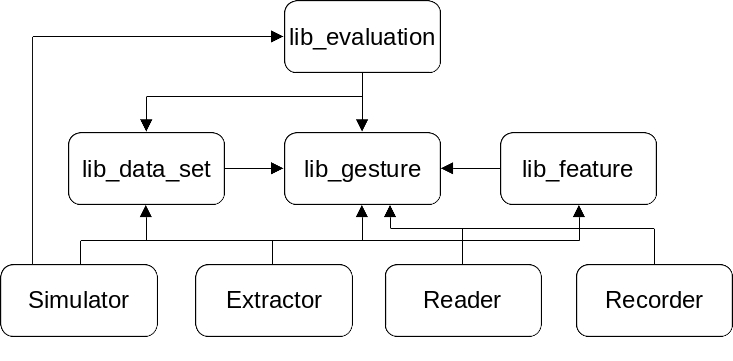
\includegraphics[width=0.75\linewidth]{images/architecture_overview.jpg}
    \caption{Abhängigkeitein der einzelnen Module.}
    \label{fig:architecture_overview}
\end{figure}
In dieser Arbeit mussten viele Features und Konfigurationen der Entscheidungsbäume untersucht und zu getestet werden. Aus diesem Grund wurde eine umfangreiche Infrastruktur geschaffen, die die
Auswertung von ML Modellen mit den Handgestendaten vereinfacht. Die Infrastruktur umfasst ein Datenmodel für Handgesten und kann die Datenmengen mit verschiedenen Parsing-Methoden einlesen.
Außerdem können synthetischen Daten auf verschiedene Arten generiert werden. Abbildung \ref{fig:architecture_overview} zeigt ein Abhängigkeitsdiagramm der einzelnen Module.
Alle Funktionalitäten wurden in Code-Bibliotheken extrahiert, um die Integration in Hilfsprogramme zu vereinfachen.
\newline
\newline
\texttt{lib\_gesture} definiert die Handgeste und die vorhandenen Handgestentypen. Außerdem implementiert sie zwei Parsing-Methoden. Die erste Methode parsed Handgesten nach Annotation und die
zweite nach Kubiks Algorithmus (Kapitel \ref{sec:gesture_extraction}). Die Handgeste implementiert Methoden, um synthetische Daten zu generieren.
\begin{itemize}
    \item Rotation um 90°, 180° und 270°.
    \item Nullgesten durch Kombination der ersten Hälfte der Ausgangshandgeste und der zweiten Hälfte von dessen Rotationen.
    \item Verschiebung der Pixel nach Oben und Unten für eine Handgeste von Links nach Rechts bzw. Rechts nach Links und analog eine Verschiebung nach Links und Rechts für eine Handgeste von Oben nach Unten bzw.
    Unten nach Oben.
    \item Rotation der äußeren Pixel, um diagonale Handgesten zu generieren.
\end{itemize}
\texttt{lib\_feature} bietet ein einfaches Interface an (Listing \ref{lst:FeatureInterface}), um Features aus einer Handgeste zu implementieren. Zurzeit sind 28 verschiedene Variationen an Features implementiert.
\begin{lstlisting}[label=lst:FeatureInterface,caption={Das Interface, um ein Feature zu implementieren.}]
pub trait Feature {
    fn calculate(gesture: &Gesture) -> Self where Self: Sized;
    fn marshal(&self) -> String;
}
\end{lstlisting}
\texttt{lib\_data\_set} stellt alle verfügbaren Datenmengen als statische Importe bereit. Einträge sind bereits nach Distanz zur Kamera, Helligkeit, Verdeckungsobjekt und Ausführungsgeschwindigkeit sortiert. Ein
Eintrag kann entweder durch einen Offset oder indem er skaliert wird in der Helligkeit verändert werden.
\newline
\newline
\texttt{lib\_evaluation} bietet ein Hilfsobjekt an, dass Datenmengen nach Klassifizierungsgenauigkeit auswertet und Berichte daraus generiert.
\newline
\newline
Der \texttt{Simulator} ist zweigeteilt. Der aktive Teil nutzt die Gestenkandidatenerkennungsmethode nach Kubik, die in \texttt{lib\_gesture} implementiert ist, um den seriellen Datenstrom des Arduino zu parsen. Der
Gestenkandidat wird anschließend durch das hinterlegte Modell klassifiziert und das Ergebnis ausgegeben. Der passive Teil evaluiert die Klassifizierungsgenauigkeit aller definierten Datenmengen mit dem momentan
hinterlegten Modell.
\newline
\newline
Der \texttt{Extractor} extrahiert aus spezifizierten Datenmengen alle definierten Features und exportiert diese in Dateien. Die können bei der Konstruktion eines Modells eingelesen werden und zum Trainieren
genutzt werden. Optional kann die Datenmenge durch synthetische Daten erweitert werden.
\newline
\newline
Der \texttt{Reader} gibt den seriellen Datenstrom des Arduino aus.
\newline
\newline
Der \texttt{Recorder} nutzt, wie der \texttt{Simulator}, den seriellen Datenstrom des Arduino und die Parsing-Methode von Kubik, um Gestenkandidaten zu erkennen.
Der Gestenkandidat wird dann in eine vordefinierte Datei reingeschrieben. Es gibt 3 Aufnahmemechanismen, um effizient Handgesten aufzunehmen.
\begin{enumerate}
    \item Es wird immer zwischen dem ausgewählten Handgestentypen und seinem inversen Handgestentypen hin und her gewechselt. Dieser Ansatz wurde von Kubik vorgeschlagen \cite{venzkeArticle}.
    \item Es kann ein fixer Handgestentyp ausgewählt werden, mit dem alle Gestenkandidaten beschriftet werden.
    \item Jedes Mal, wenn ein Gestenkandidat erkannt wurde, wird erfragt welcher Handgestentyp es ist.
\end{enumerate}